\documentclass[aspectratio=169]{beamer}

\usetheme{Madrid}
\usecolortheme{beaver}

\usepackage{amsmath, amssymb}
\usepackage{tikz}
\usetikzlibrary{arrows.meta, positioning}
\usepackage{booktabs}
\usepackage{listings}

\lstset{
  language=Python,
  basicstyle=\ttfamily\scriptsize,
  keywordstyle=\color{blue!70!black}\bfseries,
  commentstyle=\color{green!50!black}\itshape,
  stringstyle=\color{red!60!black},
  showstringspaces=false,
  breaklines=true,
  frame=single,
  columns=fullflexible,
  morekeywords={Model, quicksum, Pricer, Branchrule, Conshdlr, Sepa}
}

\title{PySCIPOpt Workshop}
\subtitle{Part 2: Advanced Techniques}
\author{PySCIPOpt Workshop}
\date{}

\begin{document}

% ---------------------------------------------------------
% Frame 1: Title
% ---------------------------------------------------------
\begin{frame}
\titlepage
\end{frame}

% ---------------------------------------------------------
% Frame 2: Roadmap
% ---------------------------------------------------------
\begin{frame}{Roadmap}
\begin{center}
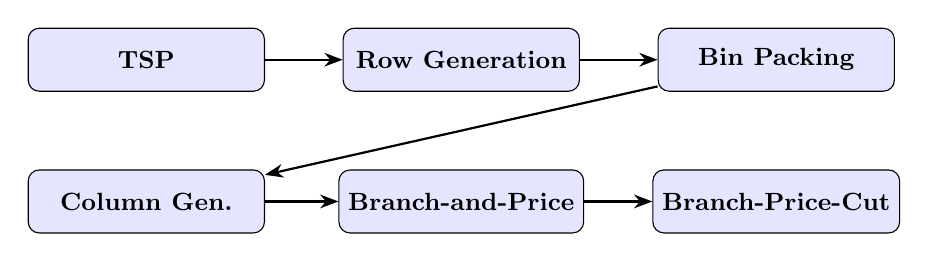
\begin{tikzpicture}[
  box/.style={draw, rounded corners, fill=blue!10, minimum width=3cm,
              minimum height=0.8cm, font=\small\bfseries},
  arr/.style={-{Stealth}, thick}
]
  \node[box] (tsp)  at (0, 0)   {TSP};
  \node[box] (row)  at (4, 0)   {Row Generation};
  \node[box] (bpp)  at (8, 0)   {Bin Packing};
  \node[box] (cg)   at (0,-1.8) {Column Gen.};
  \node[box] (bp)   at (4,-1.8) {Branch-and-Price};
  \node[box] (bpc)  at (8,-1.8) {Branch-Price-Cut};

  \draw[arr] (tsp)  -- (row);
  \draw[arr] (row)  -- (bpp);
  \draw[arr] (bpp)  -- (cg);
  \draw[arr] (cg)   -- (bp);
  \draw[arr] (bp)   -- (bpc);
\end{tikzpicture}
\end{center}

\medskip
\begin{itemize}
  \item Row generation: add \textbf{constraints} dynamically (TSP)
  \item Column generation: add \textbf{variables} dynamically (bin packing)
  \item Branch-and-price: column generation inside branch-and-bound
  \item Branch-price-and-cut: add cutting planes on top
\end{itemize}
\end{frame}

% ---------------------------------------------------------
% Frame 3: TSP Problem Statement
% ---------------------------------------------------------
\begin{frame}{Traveling Salesman Problem (TSP)}
\textbf{Given:} $n$ cities, pairwise distances $d_{ij}$

\textbf{Find:} shortest tour visiting each city exactly once, returning to start

\medskip
\begin{itemize}
  \item One of the most famous NP-hard problems
  \item Symmetric TSP: $d_{ij} = d_{ji}$ (undirected edges)
  \item We will compare two formulations:
    \begin{enumerate}
      \item Compact MTZ (polynomial constraints, weak LP)
      \item Edge formulation + SECs (exponential constraints, strong LP)
    \end{enumerate}
\end{itemize}
\end{frame}

% ---------------------------------------------------------
% Frame 4: MTZ Formulation
% ---------------------------------------------------------
\begin{frame}{MTZ Formulation}
\textbf{Variables:} $x_{ij} \in \{0,1\}$ (directed edges), $u_i \in \mathbb{R}$ (positions)

\begin{align*}
  \min \quad & \sum_{i \neq j} d_{ij}\, x_{ij} \\
  \text{s.t.} \quad
    & \sum_{j \neq i} x_{ij} = 1 && \forall\, i \quad \text{(leave once)} \\
    & \sum_{i \neq j} x_{ij} = 1 && \forall\, j \quad \text{(enter once)} \\
    & u_i - u_j + n \cdot x_{ij} \le n - 1 && \forall\, i,j \neq 0 \quad \text{(MTZ)} \\
    & x_{ij} \in \{0,1\}
\end{align*}

\begin{itemize}
  \item $O(n^2)$ variables and constraints --- no plugins needed
  \item LP relaxation is \textbf{very weak}
\end{itemize}
\end{frame}

% ---------------------------------------------------------
% Frame 5: Exercise --- Compact MTZ
% ---------------------------------------------------------
\begin{frame}{Reference: Compact MTZ}
\begin{block}{Already Implemented}
Study the MTZ formulation as a baseline before implementing row generation.
\end{block}
\begin{itemize}
  \item File: \texttt{row\_generation/compact\_mtz.py}
  \item Run: \texttt{cd row\_generation \&\& python compact\_mtz.py}
\end{itemize}
\end{frame}

% ---------------------------------------------------------
% Frame 6: Edge Formulation with SECs
% ---------------------------------------------------------
\begin{frame}{Edge Formulation with SECs}
\textbf{Variables:} $x_e \in \{0,1\}$ for each undirected edge $e$

\begin{align*}
  \min \quad & \sum_{e \in E} d_e\, x_e \\
  \text{s.t.} \quad
    & \sum_{e \in \delta(v)} x_e = 2 && \forall\, v \in V
      \quad \text{(degree)} \\
    & \sum_{e \in E(S)} x_e \le |S| - 1 && \forall\, S \subset V,\; 2 \le |S| \le n{-}1
      \quad \text{(SECs)} \\
    & x_e \in \{0,1\}
\end{align*}

\begin{itemize}
  \item \textbf{Exponentially many} SECs: $O(2^n)$ subsets
  \item \textbf{Much stronger} LP relaxation than MTZ
  \item Cannot add all upfront $\Rightarrow$ \textbf{row generation}
\end{itemize}
\end{frame}

% ---------------------------------------------------------
% Frame 7: Row Generation Paradigm
% ---------------------------------------------------------
\begin{frame}{Row Generation Paradigm}
\begin{center}
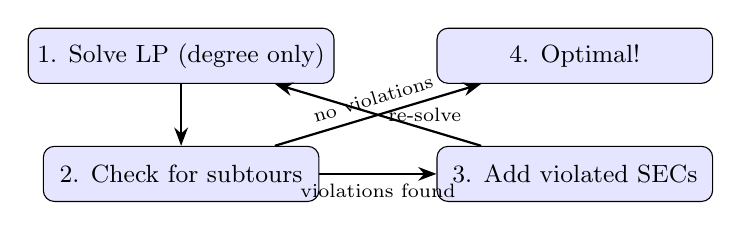
\begin{tikzpicture}[
  box/.style={draw, rounded corners, fill=blue!10, minimum width=3.5cm,
              minimum height=0.7cm, font=\small},
  arr/.style={-{Stealth}, thick}
]
  \node[box] (solve)   at (0, 0)    {1. Solve LP (degree only)};
  \node[box] (check)   at (0,-1.5)  {2. Check for subtours};
  \node[box] (add)     at (5,-1.5)  {3. Add violated SECs};
  \node[box] (opt)     at (5, 0)    {4. Optimal!};

  \draw[arr] (solve) -- (check);
  \draw[arr] (check) -- node[below, font=\scriptsize] {violations found} (add);
  \draw[arr] (add)   -- node[right, font=\scriptsize] {re-solve} (solve);
  \draw[arr] (check) -- node[above, font=\scriptsize, sloped] {no violations} (opt);
\end{tikzpicture}
\end{center}

\medskip
\begin{itemize}
  \item Start with a relaxed model (only degree constraints)
  \item Iteratively find and add violated constraints
  \item Converges to optimality without enumerating all $2^n$ SECs
\end{itemize}
\end{frame}

% ---------------------------------------------------------
% Frame 8: Constraint Handler Interface
% ---------------------------------------------------------
\begin{frame}[fragile]{Constraint Handler in SCIP}
SCIP implements row generation via the \textbf{constraint handler} plugin.

\medskip
\begin{table}
\centering\small
\begin{tabular}{lp{8cm}}
\toprule
\textbf{Callback} & \textbf{Purpose} \\
\midrule
\texttt{conscheck}  & Check if a candidate integer solution is feasible \\
\texttt{consenfolp} & Enforce constraints on LP solution; add cuts if violated \\
\texttt{conslock}   & Declare variable locks (required; can be empty) \\
\bottomrule
\end{tabular}
\end{table}

\medskip
\begin{lstlisting}
class SubtourElimination(Conshdlr):
    def conscheck(self, constraints, solution, ...):
        # Find subtours; return FEASIBLE or INFEASIBLE
    def consenfolp(self, constraints, ...):
        # Add SEC for each subtour; return CONSADDED
\end{lstlisting}
\end{frame}

% ---------------------------------------------------------
% Frame 9: Exercise --- Subtour + Conshdlr
% ---------------------------------------------------------
\begin{frame}{Exercises: Subtour Detection \& Constraint Handler}
\begin{block}{Exercise 1: Subtour Detection}
Implement \texttt{find\_subtours()} --- find connected components in the edge graph.
\end{block}
\begin{itemize}
  \item File: \texttt{row\_generation/subtour.py}
  \item Test: \texttt{python row\_generation/test\_subtour.py}
\end{itemize}

\medskip
\begin{block}{Exercise 2: Constraint Handler}
Implement \texttt{conscheck} and \texttt{consenfolp} callbacks.
\end{block}
\begin{itemize}
  \item File: \texttt{row\_generation/conshdlr\_subtour.py}
  \item Test: \texttt{python row\_generation/test\_tsp.py}
\end{itemize}
\end{frame}

% ---------------------------------------------------------
% Frame 10: Cutting Stock / Bin Packing
% ---------------------------------------------------------
\begin{frame}{Bin Packing Problem}
\textbf{Given:} items with sizes $s_i$, bins with capacity $C$

\textbf{Goal:} pack all items using the fewest bins

\medskip
\begin{itemize}
  \item NP-hard; applications in logistics, scheduling, cloud computing
  \item We will explore two formulations:
    \begin{enumerate}
      \item Compact (assignment variables) --- symmetry, weak LP
      \item Extended (pattern variables) --- column generation
    \end{enumerate}
\end{itemize}
\end{frame}

% ---------------------------------------------------------
% Frame 11: Compact Formulation
% ---------------------------------------------------------
\begin{frame}{Compact Formulation}
\textbf{Variables:} $x_{ib} \in \{0,1\}$ (item $i$ in bin $b$),
$y_b \in \{0,1\}$ (bin $b$ used)

\begin{align*}
  \min \quad & \sum_{b} y_b \\
  \text{s.t.} \quad
    & \sum_{b} x_{ib} = 1 && \forall\, i \quad \text{(assign each item)} \\
    & \sum_{i} s_i\, x_{ib} \le C\, y_b && \forall\, b \quad \text{(capacity)} \\
    & x_{ib}, y_b \in \{0,1\}
\end{align*}

\begin{itemize}
  \item \textbf{Enormous symmetry}: permuting bin indices $\Rightarrow$ equivalent solutions
  \item \textbf{Weak LP relaxation}: impractical for large instances
\end{itemize}
\end{frame}

% ---------------------------------------------------------
% Frame 12: Column Generation Idea
% ---------------------------------------------------------
\begin{frame}{Column Generation}
\begin{center}
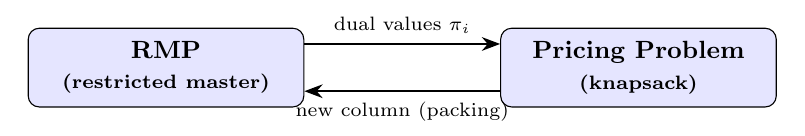
\begin{tikzpicture}[
  box/.style={draw, rounded corners, fill=blue!10, minimum width=3.5cm,
              minimum height=1cm, font=\small\bfseries, align=center},
  arr/.style={-{Stealth}, thick}
]
  \node[box] (rmp) at (0,0) {RMP\\{\scriptsize(restricted master)}};
  \node[box] (pp)  at (6,0) {Pricing Problem\\{\scriptsize(knapsack)}};

  \draw[arr, transform canvas={yshift=3mm}]
    (rmp) -- node[above, font=\scriptsize] {dual values $\pi_i$} (pp);
  \draw[arr, transform canvas={yshift=-3mm}]
    (pp) -- node[below, font=\scriptsize] {new column (packing)} (rmp);
\end{tikzpicture}
\end{center}

\medskip
\begin{enumerate}
  \item Solve RMP with small set of columns
  \item Get dual values $\pi_i$ for each covering constraint
  \item Solve pricing problem to find column with most negative reduced cost
  \item If reduced cost $\ge 0$: LP optimal. Else: add column, go to 1.
\end{enumerate}
\end{frame}

% ---------------------------------------------------------
% Frame 13: Extended Formulation
% ---------------------------------------------------------
\begin{frame}{Extended Formulation}
Let $\mathcal{P}$ = all feasible packings, $a_i^p = 1$ if item $i \in$ packing $p$:

\begin{align*}
  \min \quad & \sum_{p \in \mathcal{P}} z_p \\
  \text{s.t.} \quad
    & \sum_{p \in \mathcal{P}} a_i^p\, z_p = 1 && \forall\, i \quad \text{(cover each item)} \\
    & z_p \in \{0,1\} && \forall\, p
\end{align*}

\begin{itemize}
  \item Exponentially many packings $\Rightarrow$ cannot enumerate
  \item Column generation generates only the useful ones
  \item \textbf{Stronger LP relaxation} than compact formulation
\end{itemize}
\end{frame}

% ---------------------------------------------------------
% Frame 14: Pricing = Knapsack
% ---------------------------------------------------------
\begin{frame}{Pricing Problem = Knapsack}
Reduced cost of a new packing $a$:
\[
  \bar{c} = 1 - \sum_{i} a_i \pi_i
\]

Minimize reduced cost subject to capacity:
\begin{align*}
  \min \quad & 1 - \sum_{i} a_i\, \pi_i \\
  \text{s.t.} \quad
    & \sum_{i} s_i\, a_i \le C \\
    & a_i \in \{0,1\}
\end{align*}

Equivalently: $\max \sum_i a_i \pi_i$ s.t.\ capacity $\Rightarrow$ \textbf{0--1 knapsack}!

\medskip
When optimal reduced cost $\ge 0$: no improving column exists.
\end{frame}

% ---------------------------------------------------------
% Frame 15: Pricer Plugin
% ---------------------------------------------------------
\begin{frame}[fragile]{Pricer Plugin in SCIP}
\begin{table}
\centering\small
\begin{tabular}{lp{8cm}}
\toprule
\textbf{Callback} & \textbf{Purpose} \\
\midrule
\texttt{pricerredcost} & Generate columns with negative reduced cost \\
\texttt{pricerfarkas}  & Generate columns to restore feasibility \\
\bottomrule
\end{tabular}
\end{table}

\medskip
\begin{lstlisting}
class KnapsackPricer(Pricer):
    def pricerredcost(self):
        duals = {i: self.model.getDualsolLinear(cons)
                 for i, cons in self.constraints.items()}
        red_cost, pattern = solve_knapsack(...)
        if red_cost < -1e-6:
            new_var = self.model.addVar(
                vtype="B", obj=1, pricedVar=True)
            # Add coefficients to covering constraints
        return {"result": SCIP_RESULT.SUCCESS}
\end{lstlisting}
\end{frame}

% ---------------------------------------------------------
% Frame 16: Exercise --- Pricing
% ---------------------------------------------------------
\begin{frame}{Exercise: Knapsack Pricing}
\begin{block}{Task}
Implement the 0--1 knapsack solver used as the pricing subproblem.
Return \texttt{(optimal\_value, list\_of\_selected\_items)}.
\end{block}
\begin{itemize}
  \item File: \texttt{branch\_and\_price/pricing\_knapsack.py}
  \item Test: \texttt{cd branch\_and\_price \&\& python test\_pricing\_knapsack.py}
\end{itemize}
\end{frame}

% ---------------------------------------------------------
% Frame 17: Why Standard Branching Fails
% ---------------------------------------------------------
\begin{frame}{Why Standard Branching Fails}
Standard variable branching on $z_p$:

\medskip
\begin{columns}[T]
\begin{column}{0.48\textwidth}
\begin{block}{$z_p = 1$}
Force \emph{one specific} packing out of exponentially many.

$\Rightarrow$ \textbf{Very restrictive}
\end{block}
\end{column}
\begin{column}{0.48\textwidth}
\begin{block}{$z_p = 0$}
Forbid \emph{one specific} packing out of exponentially many.

$\Rightarrow$ \textbf{Barely restrictive}
\end{block}
\end{column}
\end{columns}

\bigskip
\begin{center}
Result: \textbf{highly unbalanced} branch-and-bound tree

$\Rightarrow$ Very slow convergence
\end{center}
\end{frame}

% ---------------------------------------------------------
% Frame 18: Ryan-Foster Branching
% ---------------------------------------------------------
\begin{frame}{Ryan-Foster Branching}
Branch on \textbf{pairs of items} $(i, j)$ instead of individual variables:

\medskip
\begin{columns}[T]
\begin{column}{0.48\textwidth}
\begin{block}{Together}
Items $i$ and $j$ must be in the \textbf{same} bin.
\end{block}
\end{column}
\begin{column}{0.48\textwidth}
\begin{block}{Apart}
Items $i$ and $j$ must be in \textbf{different} bins.
\end{block}
\end{column}
\end{columns}

\bigskip
\textbf{How to find a pair:}
\begin{itemize}
  \item Compute implicit pair variable: $x_{ij} = \sum_{p:\, i \in p,\, j \in p} z_p$
  \item Choose pair where $0 < x_{ij} < 1$ (fractional)
\end{itemize}

\medskip
$\Rightarrow$ Much more \textbf{balanced} search tree
\end{frame}

% ---------------------------------------------------------
% Frame 19: Exercise --- Ryan-Foster
% ---------------------------------------------------------
\begin{frame}{Exercises: Ryan-Foster Branching}
\begin{block}{Exercise: Fractional Pairs}
Implement \texttt{all\_fractional\_pairs()} --- find all item pairs with fractional implicit values.
\end{block}
\begin{itemize}
  \item File: \texttt{branch\_and\_price/ryan\_foster.py}
  \item Test: \texttt{cd branch\_and\_price \&\& python test\_fractional\_pairs.py}
\end{itemize}

\medskip
\begin{block}{Exercise: Branching Decisions}
Complete the child-node creation logic: inherit parent decisions, add new pair.
\end{block}
\begin{itemize}
  \item File: \texttt{branch\_and\_price/ryan\_foster.py}
\end{itemize}
\end{frame}

% ---------------------------------------------------------
% Frame 20: Enforcing Branching in Pricing
% ---------------------------------------------------------
\begin{frame}[fragile]{Enforcing Branching in Pricing}
The pricing problem must respect \textbf{all} accumulated branching decisions:

\medskip
\begin{itemize}
  \item \textbf{Together} $(i, j)$: add constraint $a_i = a_j$ in knapsack
  \item \textbf{Apart} $(i, j)$: add constraint $a_i + a_j \le 1$ in knapsack
\end{itemize}

\medskip
\begin{lstlisting}
# Together constraints
for i, j in together:
    m.addCons(x[i] == x[j])

# Apart constraints
for i, j in apart:
    m.addCons(x[i] + x[j] <= 1)
\end{lstlisting}

\medskip
\textbf{Note:} Apart does not forbid both items being \emph{absent}.
\end{frame}

% ---------------------------------------------------------
% Frame 21: Exercise --- Constrained Pricing
% ---------------------------------------------------------
\begin{frame}{Exercise: Constrained Pricing}
\begin{block}{Task}
Implement \texttt{solve\_knapsack\_with\_constraints()} --- extend the knapsack solver
with together/apart constraints from Ryan-Foster branching.
\end{block}
\begin{itemize}
  \item File: \texttt{branch\_and\_price/pricing\_knapsack.py}
  \item Test: \texttt{cd branch\_and\_price \&\& python test\_knapsack\_with\_constraints.py}
\end{itemize}

\medskip
\begin{block}{Integration Test}
After all B\&P exercises: \texttt{cd branch\_and\_price \&\& python test\_bnp.py}
\end{block}
\end{frame}

% ---------------------------------------------------------
% Frame 22: Branch-Price-and-Cut
% ---------------------------------------------------------
\begin{frame}{Branch-Price-and-Cut}
Strengthen branch-and-price by adding \textbf{cutting planes}:

\medskip
\textbf{Subset-row inequalities} for set partitioning:

For any triple of items $S = \{i, j, k\}$, consider all packings covering
$\ge 2$ items in $S$. If their LP values sum $> 1$:
\[
  \sum_{p:\, |p \cap S| \ge 2} z_p \le 1
\]

\medskip
\textbf{Separator plugin} in SCIP:
\begin{itemize}
  \item \texttt{sepaexeclp}: search for violated inequalities at each LP solution
  \item Return \texttt{SEPARATED} if cut added, \texttt{DIDNOTFIND} otherwise
\end{itemize}
\end{frame}

% ---------------------------------------------------------
% Frame 23: Exercise --- Subset-Row Separator
% ---------------------------------------------------------
\begin{frame}{Exercise: Subset-Row Separator}
\begin{block}{Task}
Implement the subset-row separator: enumerate triples of fractional
LP variables and add cuts when their values sum exceeds 1.
\end{block}
\begin{itemize}
  \item File: \texttt{separator/subset\_row/subset\_row.py}
  \item Test: \texttt{cd separator/subset\_row \&\& python test\_subset\_row.py}
\end{itemize}
\end{frame}

% ---------------------------------------------------------
% Frame 24: Summary
% ---------------------------------------------------------
\begin{frame}{Summary \& Further Resources}
\textbf{What we covered:}
\begin{itemize}
  \item TSP: compact MTZ vs.\ row generation with SECs
  \item Bin packing: compact vs.\ extended formulation
  \item Column generation with knapsack pricing
  \item Branch-and-price with Ryan-Foster branching
  \item Branch-price-and-cut with subset-row inequalities
\end{itemize}

\medskip
\textbf{Bonus exercises} (see \texttt{branch\_and\_price/README.md}):
\begin{itemize}
  \item Dual stabilization, Lagrangian bound
  \item Better initialization, faster pricing
  \item Handling numerical issues
\end{itemize}

\medskip
\textbf{Resources:}
\begin{itemize}
  \item \url{https://www.scipopt.org/} --- SCIP documentation
  \item \url{https://github.com/scipopt/PySCIPOpt} --- PySCIPOpt
\end{itemize}
\end{frame}

\end{document}
